\documentclass[handout,nooutcomes]{ximera}
%% handout
%% space
%% newpage
%% numbers
%% nooutcomes


\newcommand{\RR}{\mathbb R}
\renewcommand{\d}{\,d}
\newcommand{\dd}[2][]{\frac{d #1}{d #2}}
\renewcommand{\l}{\ell}
\newcommand{\ddx}{\frac{d}{dx}}
\newcommand{\dfn}{\textbf}
\newcommand{\eval}[1]{\bigg[ #1 \bigg]}

\usepackage{multicol}

\renewenvironment{freeResponse}{
\ifhandout\setbox0\vbox\bgroup\else
\begin{trivlist}\item[\hskip \labelsep\bfseries Solution:\hspace{2ex}]
\fi}
{\ifhandout\egroup\else
\end{trivlist}
\fi} %% we can turn off input when making a master document

\title{Recitation \#1 Chapter 1 - Precalculus Review}  

\begin{document}
\begin{abstract}		\end{abstract}
\maketitle

\section*{Warm up:}
   
If $f$ is always increasing, is $f^{-1}$ always increasing?

			 \begin{freeResponse}		 
			Yes, if $f$ is always increasing, then $f^{-1}$ is always increasing.  To prove this, suppose $x < y$.  Then it follows from the definition of $f^{-1}$ that $f(f^{-1}(x)) = x < y =  f(f^{-1}(y))$.  But since $f$ is increasing, this implies that $f^{-1}(x)  < f^{-1}(y)$.	
			\end{freeResponse}


\section*{Group work:}
	\begin{problem}
	 	Given the graph of the function $f$ below, answer the following questions.
			
\begin{image}		
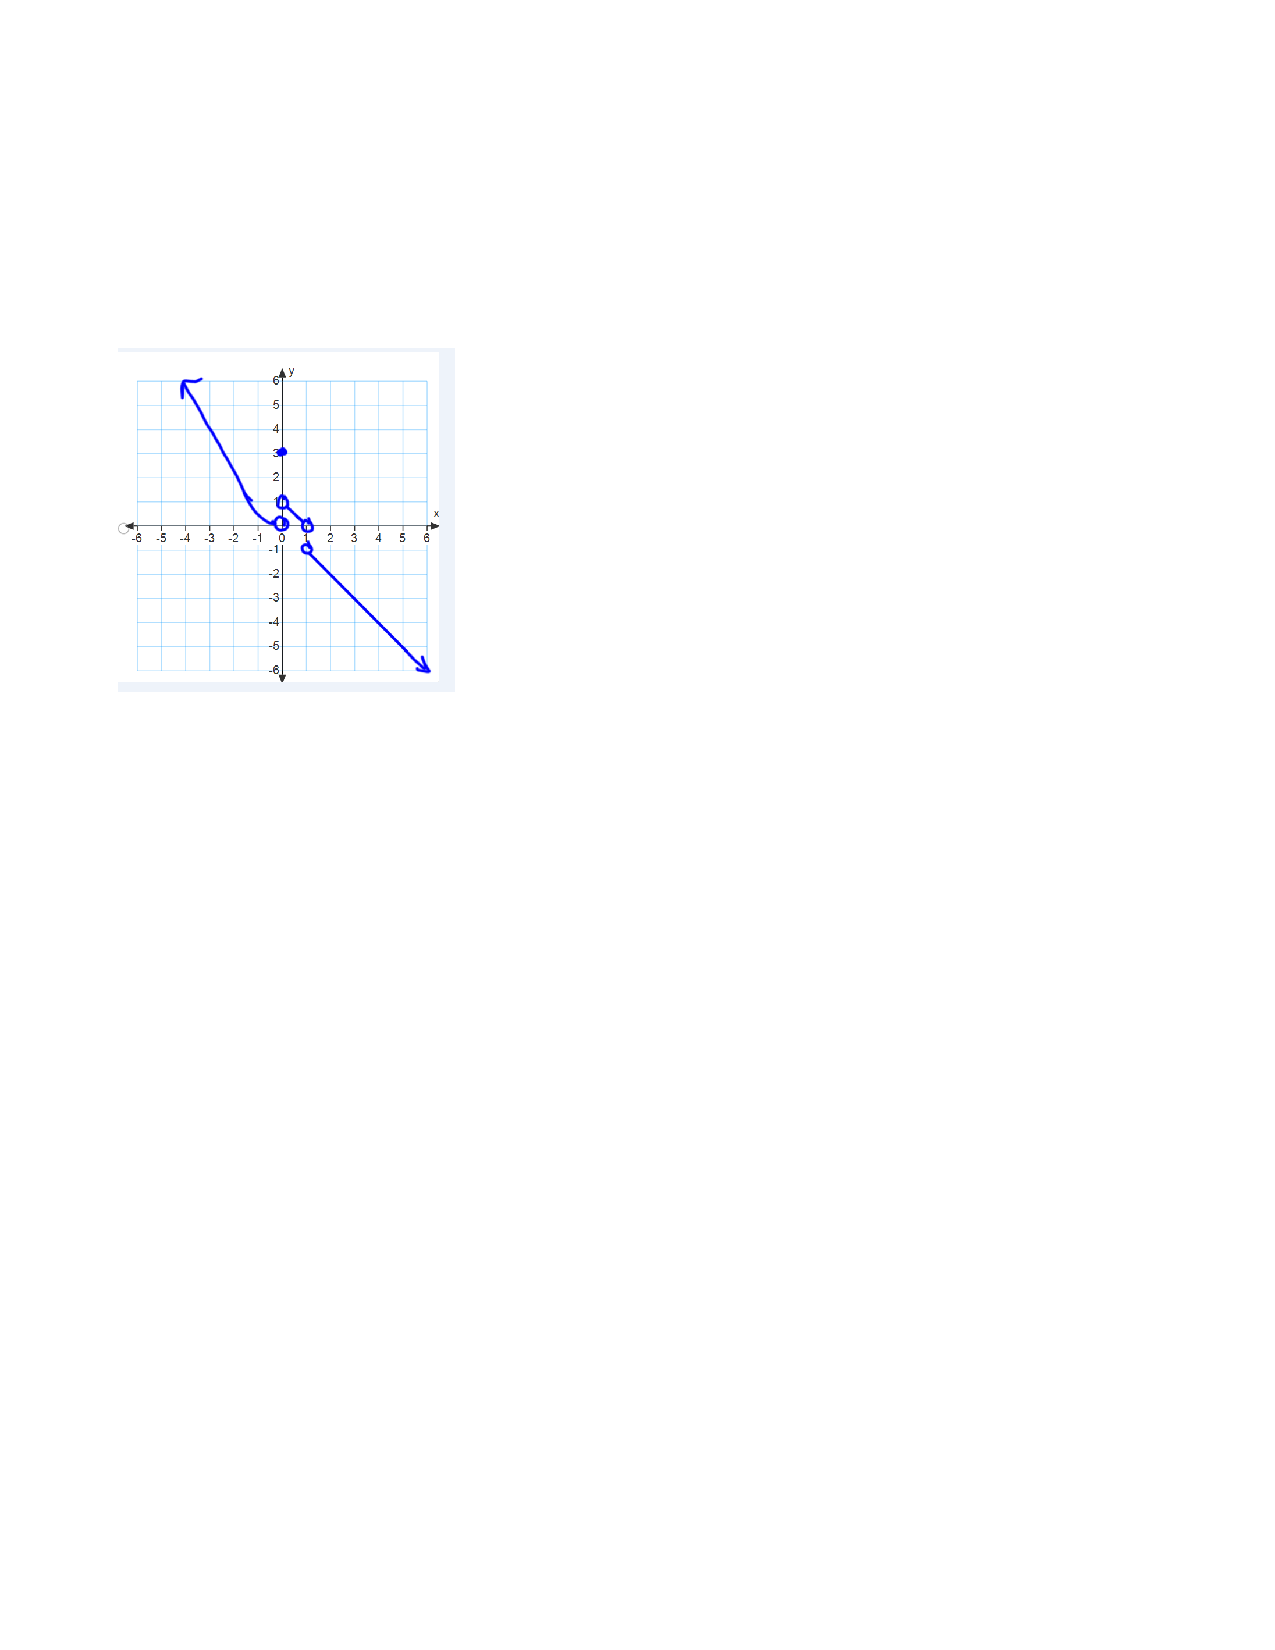
\includegraphics[trim= 80 460 300 170]{Figure3.pdf}
\end{image}	

		\begin{enumerate}
		
			 \item What is the domain of $f$?
			 
			 \begin{freeResponse}			 
			 $(-\infty, 1) \cup (1, \infty)$
			\end{freeResponse}
			 
			 \item What is the range of $f$?
			 
			 \begin{freeResponse}			 
			 The range is $(-\infty ,-1) \cup (0,\infty )$
			 \end{freeResponse}
			 
			 \item What is $f(0)$?  $f(1)$?  $f(2)$?
			 
			  \begin{freeResponse}			 
			 $f(0)=3$, $f(1)$ does not exist, $f(2)=-2$
			 \end{freeResponse}
			 
			 \item Does $f$ have an inverse?  Why or why not?
			 
			  \begin{freeResponse}			 
			 No, the function does not have an inverse.  It is not one-to-one (ie, it does not pass the horizontal line test).
			 \end{freeResponse}
			
			\end{enumerate}
			
	\end{problem}
	
\begin{problem}			
				
Find the inverse $y=f^{-1}(x)$ of the function.  State the domain and range of the inverse.
	
			\begin{enumerate}
			\item  $f(x)=x^2-4x-5$ (when $x\geq2$).
			
			 \begin{freeResponse}			 
			 $f(x)= y =x^2-4x-5 $ 
			
			$y-5=x^2-4x $
			
			complete the square
			
			$y+5+4=x^2-4x+4 = (x-2)^2$
			
			$ \sqrt{y+9}=x-2$
			
			$2+\sqrt{y+9}=x$
			
			$f^{-1}(x) = 2 + \sqrt{x + 9}$
			
			The domain of $f^{-1}(x)$ is $[-9,\infty )$.  The range is $[2,\infty )$.
			 \end{freeResponse}
			 
			\item  $f(x)=\sqrt[4]{x+2}$.
			
			 \begin{freeResponse}			 
			 $y=\sqrt[4]{x+2}$
			
			$y^4 = x + 2$
			
			$y^4 - 2 = x$
			
			$f^{-1}(x) = x^4 - 2$
			
			The domain of $f^{-1}(x)$ is $[0, \infty )$.  The range is $[-2, \infty )$.  
			 \end{freeResponse}
			 
			\item  $f(x)=\frac{1}{(x+2)^2}$  (when $x>-2$).
			
			 \begin{freeResponse}			 
			 $y = \frac{1}{(x+2)^2}$
			
			$(x+2)^2 = \frac{1}{y}$
			
			$ x+2 = \sqrt{\frac{1}{y}} = \frac{1}{\sqrt{y}}$	
			
			$x = \frac{1}{\sqrt{y}} - 2 $
			
			$f^{-1}(x) = \frac{1}{\sqrt{x}} - 2$
			
			The domain of $f^{-1}(x)$ is $(0, \infty)$.  The range is $(-2, \infty )$. 
			 \end{freeResponse}
			 
			\end{enumerate}
			
\end{problem}
	
	
	
\begin{problem}
Find all values of $x$ which satisfy the equation.
	
			\begin{enumerate}
			
			\item  $\log_x 25=2$ 
			
			 \begin{freeResponse}			 
			 $x^2 = 25 \, \Longrightarrow \, x = \pm 5$.  But the base of a logarithm is always a positive number different from 1, and therefore $x = 5$ is the only solution. 
			 \end{freeResponse}
			
			\item  $7^x=15$ 
			
			 \begin{freeResponse}			 
			 $x = \log_{7} 15$. 
			 \end{freeResponse}
			
			\end{enumerate}
			
\end{problem}
			
			

\begin{problem}
Find all values which satisfy the given equation.
	
			\begin{enumerate}
			
			\item  $\cos (x)=1$ 
			
			 \begin{freeResponse}			 
			 This is asking for the angles such that cosine of that angle equals 1.  Thus, $x = 2 \pi n$, where $n$ is any integer.  
			 \end{freeResponse}
			
			\item  $\sin (3 \theta )=\frac{\sqrt{3}}{2}$ for $0 \leq \theta \leq 2\pi $
			
			 \begin{freeResponse}			 
			 Let $3 \theta = x$, so that we have that 
			
			$ \frac{\sqrt{3}}{2} = \sin(x) $.
			
			So $ x= \frac{\pi}{3} + 2 \pi n$ or $ x = \frac{2 \pi }{3} + 2 \pi n $ for $n$ any integer.  Since $x = 3 \theta$, we can solve for theta to obtain $ \theta = \frac{\pi}{9} + \frac{2}{3} \pi n $ or $ \theta = \frac{2 \pi }{9} + \frac{2}{3} \pi n $, where $n$ is again any integer.  
			
We are only looking for solutions of $\theta$ in $[0, 2 \pi ]$, and so our solutions are

$ \theta = \frac{\pi}{9}, \frac{2\pi}{9}, \frac{7\pi}{9}, \frac{8\pi}{9}, \frac{13\pi}{9}, \frac{14\pi}{9} $ 
			 \end{freeResponse}
			
			\end{enumerate}
			
\end{problem}
			
			
			
\begin{problem}
	
			\begin{enumerate}
			
			\item  Simplify the expression:  $\cos^{-1} \left( \sin \left( \frac{\pi }{2} \right) \right) $ 
			
			 \begin{freeResponse}			 
			 $ \sin \left( \frac{\pi}{2} \right) = 1$, and so we are looking for $\cos^{-1}(1)$.  The range of $\cos^{-1}$ is $[0, \pi]$, and so $\cos^{-1} (1) = 0$.  
			 \end{freeResponse}
			 
			 
			 
			 
			 
			 
			
			\item  Simplify the expression:  $ \tan \left( \sin^{-1} \left( \frac{4}{x} \right) \right) $ 
			
			 \begin{freeResponse}			 
			 Let $\theta = \sin^{-1} \left( \frac{4}{x} \right) $.  Then $\sin \theta = \frac{4}{x}$.  Consider the corresponding right triangle
			 
			 \begin{image}
			 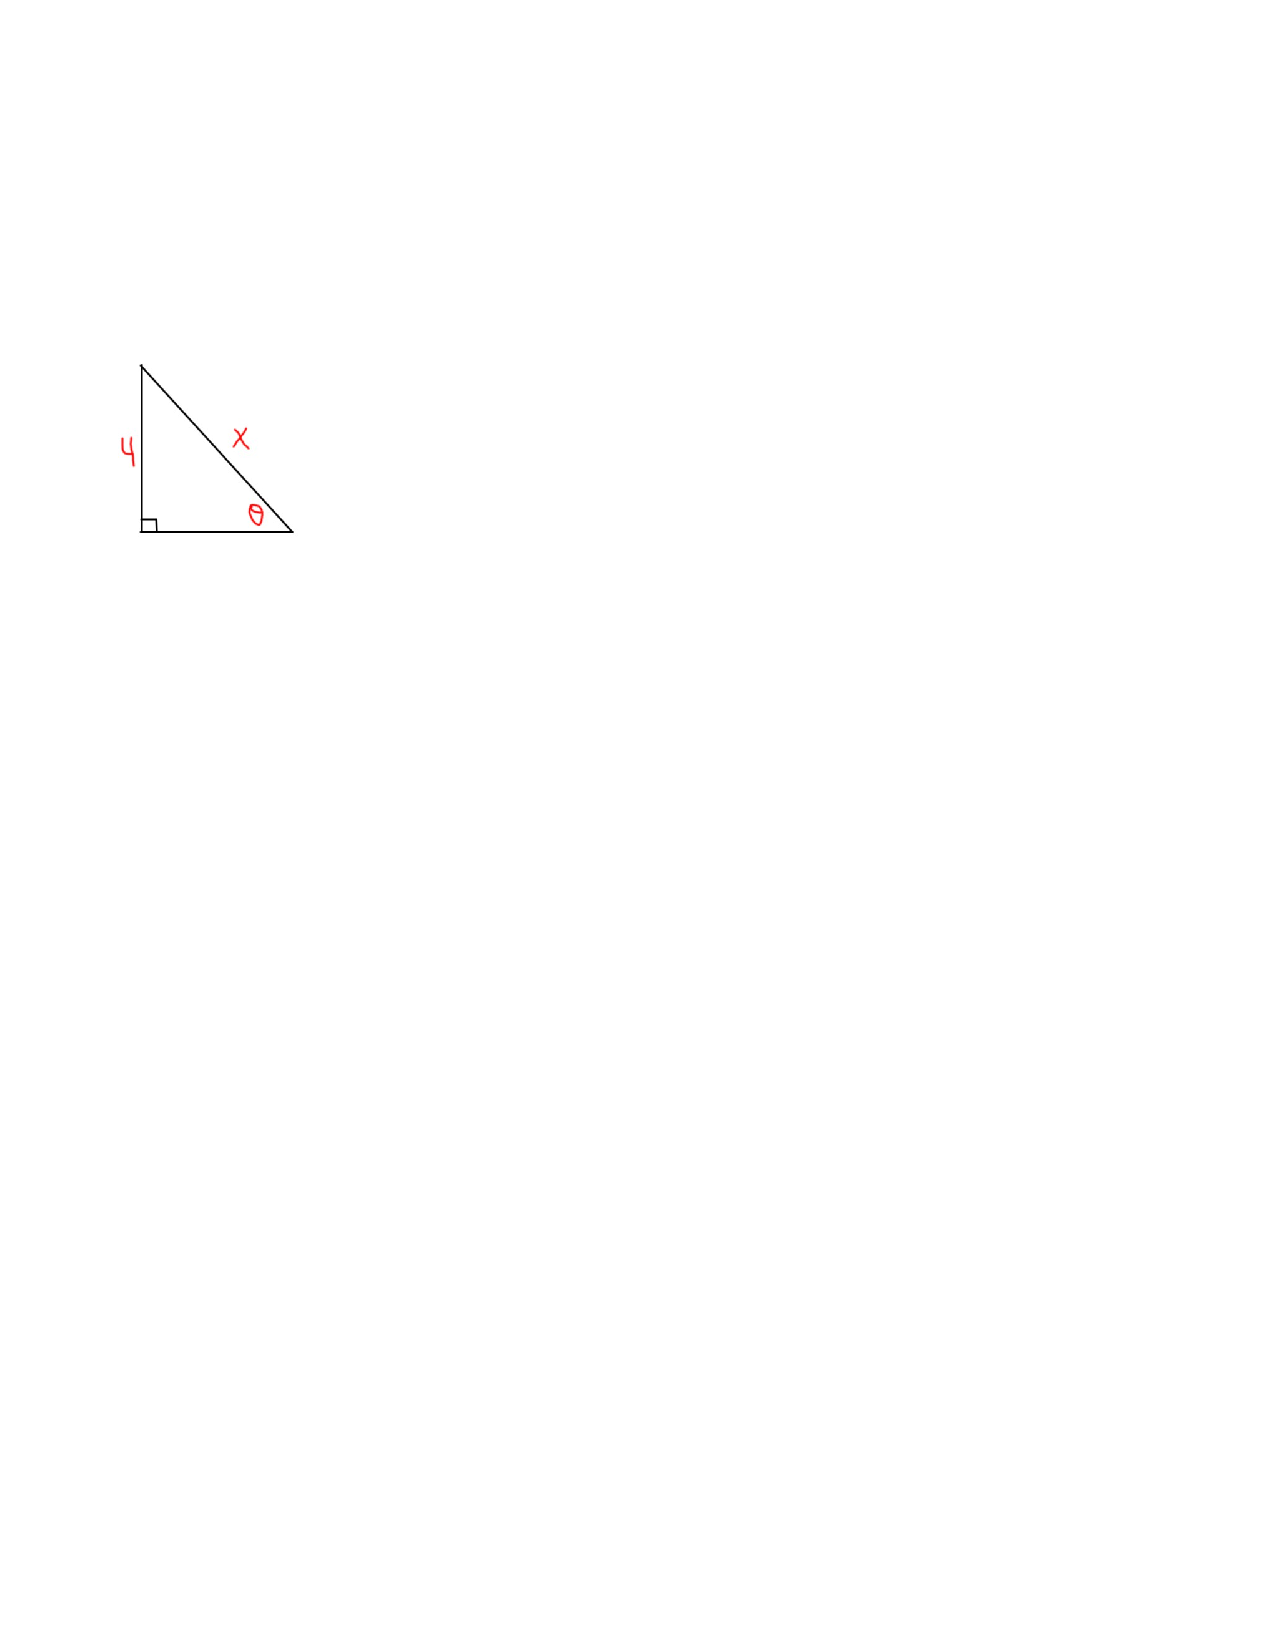
\includegraphics[trim=60 525 300 170]{Figure5.pdf}
			 \end{image}
			 Call the adjacent side $y$.  We use the Pythagorean Theorem to obtain
			
			$x^2 = 16 + y^2 \Longrightarrow y = \sqrt{x^2 - 16}$.
			
			Then
			
			$ \tan \left( \sin^{-1} \left( \frac{4}{x} \right) \right) = \tan \theta = \frac{4}{y} = \frac{4}{\sqrt{x^2 - 16}}  $.
			 \end{freeResponse}
			
			\end{enumerate}
			
\end{problem}
			
			
			

	










								
				
				
	



























\end{document} 


















